% !TeX program = xelatex
% !TeX encoding = UTF-8
% !TeX spellcheck = en_US
% !BIB program = biber
%% 
%% The above lines help editors like TeXstudio to automatically choose the right tools
%% to compile your LaTeX source file. If your tool does not support these magic comments,
%% you will need to make appropriate manual choices.
%% 
%% You can safely use "pdflatex" instead of "xelatex" if you prefer the pdfLaTeX toolchain.
%% However, pdfLaTeX will not be able to deliver the professional font experience that you
%% will get with XeLaTeX. You can also safely use "lualatex" instead of "xelatex" while
%% preserving the professional font experience if you prefer the LuaLaTeX toolchain.
%% 
%% _Important_: These magic comments should be on the first lines of your source file.
%% 
%%%%%%%%%%%%%%%%%%%%%%%%%%%%%%%%%%%%%%%%%%%%%%%%%%%%%%%%%%%%%%%%%%%%%%%%%%%%%%%%

%%%%%%%%%%%%%%%%%%%%%%%%%%%%%%%%%%%%%%%%%%%%%%%%%%%%%%%%%%%%%%%%%%%%%%%%%%%%%%%%
%% 
%%            JJJJ   K                         K   UUUU         UUUU  
%%            JJJJ   KKKK                   KKKK   UUUU         UUUU  
%%            JJJJ   KKKKKK               KKKKKK   UUUU         UUUU  
%%            JJJJ      KKKKKK         KKKKKK      UUUU         UUUU  
%%            JJJJ         KKKKKK   KKKKKK         UUUU         UUUU  
%%            JJJJ            KKKKKKKKK            UUUU         UUUU  
%%    JJ     JJJJJ               KKK               UUUUU       UUUUU  
%%  JJJJJJJJJJJJJ    KKKKKKKKKKKKKKKKKKKKKKKKKKK    UUUUUUUUUUUUUUU   
%%    JJJJJJJJJ      KKKKKKKKKKKKKKKKKKKKKKKKKKK      UUUUUUUUUUU     
%% 
%% This is an example file for using the JKU LaTeX technical report template
%% for your technical report.
%% 
%% Template created by Michael Roland (2021)
%% 
%%%%%%%%%%%%%%%%%%%%%%%%%%%%%%%%%%%%%%%%%%%%%%%%%%%%%%%%%%%%%%%%%%%%%%%%%%%%%%%%

%%%%%%%%%%%%%%%%%%%%%%%%%%%%%%%%%%%%%%%%%%%%%%%%%%%%%%%%%%%%%%%%%%%%%%%%%%%%%%%%
%% 
%% Document class: This is a koma-script article.
%% 
\documentclass[a4paper,oneside,11pt,ngerman,english]{scrartcl}
%% 
%% The comma-separated list in square brackets are class options.
%% Useful options that you might want to use:
%% 
%% Paper size:
%%  * a4paper ... A4 paper size
%% 
%% Optimize for single-sided or double-sided printing:
%%  * oneside ... single-sided
%%  * twoside ... double-sided
%% 
%% Base font size:
%%  * 10pt ... 10-pt font is used for normal text
%%  * 11pt ... 11-pt font is used for normal text
%% 
%% Define document languages (the last specified language becomes the document default
%% language):
%%  * ngerman ... German
%%  * english ... English
%%  * ...
%% 
%% Alternate document classes: The JKU report template supports the koma-script classes
%% `scrartcl', `scrreprt' and `scrbook'. The article class `scrartcl' is well-suited
%% for a typical technical report. However, `scrbook' or `scrreprt' may be better
%% suited for longer reports since they permit structuring your work in chapters.
%%  
%% _Important_: The document class should be the first line of LaTeX code in your main
%% source file. Do not place anything but comments / magic comments above that line (unless
%% you really know what you are doing).
%% 
%%%%%%%%%%%%%%%%%%%%%%%%%%%%%%%%%%%%%%%%%%%%%%%%%%%%%%%%%%%%%%%%%%%%%%%%%%%%%%%%

%%%%%%%%%%%%%%%%%%%%%%%%%%%%%%%%%%%%%%%%%%%%%%%%%%%%%%%%%%%%%%%%%%%%%%%%%%%%%%%%
%% 
%% Treat input files as UTF-8 encoded. Make sure to always load this when you use pdfLaTeX
%% so that pdfLaTeX knows how to read and interpret characters in this source file.
%% 
\usepackage[utf8]{inputenc}
%% 
%%%%%%%%%%%%%%%%%%%%%%%%%%%%%%%%%%%%%%%%%%%%%%%%%%%%%%%%%%%%%%%%%%%%%%%%%%%%%%%%

%%%%%%%%%%%%%%%%%%%%%%%%%%%%%%%%%%%%%%%%%%%%%%%%%%%%%%%%%%%%%%%%%%%%%%%%%%%%%%%%
%% 
%% Use the JKU LaTeX technical report template for this document.
%% 
\usepackage[TNF,equalmargins,techreport,fancyfonts]{jkureport}
%% 
%% The comma-separated list in square brackets are theme options. Useful options that you
%% might want to use:
%% 
%% Document type:
%%  * phdthesis     ... PhD thesis.
%%  * mathesis      ... Master's thesis.
%%  * diplomathesis ... Diploma thesis.
%%  * bathesis      ... Bachelor's thesis.
%%  * seminarreport ... Seminar report.
%%  * techreport    ... Technical report.
%% 
%% Color scheme selection options:
%%  * JKU  ... Use JKU (gray) color scheme (this is the default if no scheme is selected).
%%  * BUS  ... Use Business School color scheme.
%%  * LIT  ... Use Linz Institute of Technology color scheme.
%%  * MED  ... Use MED faculty color scheme.
%%  * RE   ... Use RE faculty color scheme.
%%  * SOE  ... Use School of Education color scheme.
%%  * SOWI ... Use SOWI faculty color scheme.
%%  * TNF  ... Use TNF faculty color scheme.
%% 
%% Space-efficient monospace font options (requires XeTeX/LuaTeX):
%%  * compactmono   ... Use condensed fixed-width font everywhere.
%%  * nocompactverb ... Do not use condensed fixed-width font for verbatim and listings.
%% 
%% Style-breaking options:
%%  * noimprint      ... Do not insert imprint on title pages.
%%  * nojkulogo      ... Do not insert JKU & K logos on title pages.
%%  * capstitle      ... Set document title in capital letters.
%%  * nofancyfonts   ... Do not use custom TTF fonts with XeTeX/LuaTeX / supress pdfLaTeX warning.
%%  * equalmargins   ... Decrease the outer page margin to have both page margins of equal size
%%                       (the additional outer margin is intentional and to be used for
%%                       anotations; equalmargins also causes the text width to be
%%                       significantly larger than optimal for reading).
%% 
%% Experimental options:
%%  * mathastext ... Use standard document fonts (enhanced with symbols from Fira Math font
%%                   when using XeTeX/LuaTeX) in math mode.
%% 
%% Advanced options:
%%  * noautopdfinfo     ... Do not automatically try to add pdfinfo with hyperref from document
%%                          metadata fields.
%%  * logopath={<path>} ... Set the path where the theme can find its own logo resources. This
%%                          should typically be a relative path and the default is `./logos'.
%%  * fontpath={<path>} ... Set the path where the theme can find its own font resources. This
%%                          should typically be a relative path and the default is `./fonts'.
%% 
%% Hint: Boolean options can be used in the forms `option' or `option=true' the enable the
%% option and `nooption' or `option=false' to disable the option.
%% 
%%%%%%%%%%%%%%%%%%%%%%%%%%%%%%%%%%%%%%%%%%%%%%%%%%%%%%%%%%%%%%%%%%%%%%%%%%%%%%%%

%%%%%%%%%%%%%%%%%%%%%%%%%%%%%%%%%%%%%%%%%%%%%%%%%%%%%%%%%%%%%%%%%%%%%%%%%%%%%%%%
%% 
%% This is the place where you can load additional packages. If you want to load
%% a package `biblatex', you would use the command `\usepackage{biblatex}'.
%% 
\usepackage{amsfonts, amsmath}
\usepackage{subfigure}
\usepackage{listings}
\usepackage{caption}

\captionsetup{
    margin=10pt,
    font=small,
    labelfont=bf,
    justification=raggedleft
}
\lstset{
    language=vhdl
}
\captionsetup[lstlisting]{position=above}
\newcommand{\vhdl}[1]{\lstinline!#1!}

%% 
%%%%%%%%%%%%%%%%%%%%%%%%%%%%%%%%%%%%%%%%%%%%%%%%%%%%%%%%%%%%%%%%%%%%%%%%%%%%%%%%

\begin{document}
%%%%%%%%%%%%%%%%%%%%%%%%%%%%%%%%%%%%%%%%%%%%%%%%%%%%%%%%%%%%%%%%%%%%%%%%%%%%%%%%
%% 
%% Report information and title page
%% 

%% Command \title{title}: sets the title of your report
\title{01 - VHDL Exercise}

%% Command \titleshort{short title}: sets an abbreviated version of the report title for page heads
%\titleshort{Optional space for your abbreviated title}

%% Command \subtitle{subtitle}: sets the subtitle for seminar/technical reports (not used for theses)
\subtitle{Hardwaredesign PR - Exercise 01\\%
    \usekomafont{subtitlesmall}%
    \hfill\\%
    Semester 2024W\\
    \hfill\\%
}

%% Command \author{name}: sets the author name(s); separate multiple authors with \and; use \prefix{}
%%   and \suffix{} to add academic titles and suffixes (if needed); use \affiliation{} to add an
%%   affiliation, use \authornewline to add line breaks (e.g. to separate authors from contact
%%   information), use \authormail{}, \authorweb{}, \authorphone{} and \authorfax{} to add contact
%%   information)
\author{%
    Simon Grundner
    \affiliation{Institute for Signal Processing}
    \authornewline
    \authormail{k12136610@students.jku.at}
    \authorweb{https://jku.at/isp}
    \authornewline
}

%% Command \date{YYYY-MM-DD}: set the day of publication (defaults to today)
%\date{2020-04-09}

%% Command \partnerlogo{filename}: use filename as partnerlogo, filename may be blank to disable the logo
\partnerlogo{logos/isp}

%% Command \revisionblock{text}: set the document revision block on the title page
%\revisionblock{Space for your revision block, acknowledgements, etc.}

%% Command \reportnumber{number}: set the report number
%\reportnumber{Space for your report number}

%% Command \setbottommark{text}: set the bottom mark (in document footer)
\setbottommark{Simon Grundner, k12136610}

%% Command \abstract{text}: set the document abstract on the title page
%\abstract{Space for your (short) abstract.}

%% Command \keywords{text}: set the document keywords
\keywords{Combinatorial Circuits, Adder}


%% Finally, print the title page using the above information:
\maketitle
%% 
%%%%%%%%%%%%%%%%%%%%%%%%%%%%%%%%%%%%%%%%%%%%%%%%%%%%%%%%%%%%%%%%%%%%%%%%%%%%%%%%

%%%%%%%%%%%%%%%%%%%%%%%%%%%%%%%%%%%%%%%%%%%%%%%%%%%%%%%%%%%%%%%%%%%%%%%%%%%%%%%%
%% 
%% Add a table of contents
%% 

%% Print the table of contents
\tableofcontents

%% Make sure to start the list of acronyms on a new odd page (odd is only relevant in twoside layout)
%\cleardoubleoddpage
%% Include list of acronyms (optional and often not necessary)
%\import{./}{acronyms}

%% 
%%%%%%%%%%%%%%%%%%%%%%%%%%%%%%%%%%%%%%%%%%%%%%%%%%%%%%%%%%%%%%%%%%%%%%%%%%%%%%%%

%%%%%%%%%%%%%%%%%%%%%%%%%%%%%%%%%%%%%%%%%%%%%%%%%%%%%%%%%%%%%%%%%%%%%%%%%%%%%%%%
%% 
%% Add your report sections ...
%% 

\section{Combinatorial Circuit}\label{section:combinatorial-circuit}

\begin{highlightblock}[Combinatorial Circuit]
Write an entity and architecture for the system described in Figure \ref{fig:comb}. This entity has two inputs (\vhdl{operand_a_i} and \vhdl{operand_b_i}) and two outputs. The first output \vhdl{and_o} should be calculated as the logical AND operation of the two inputs and the second output \vhdl{or_o} should be calculated as the logical OR operation of the two inputs.

\begin{center}
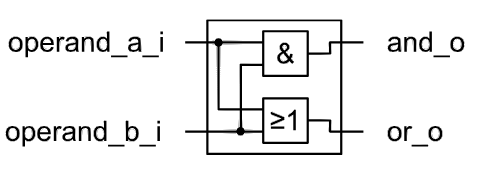
\includegraphics[width=0.5\linewidth]{images/combinatorial-circuit.png}

Figure \refstepcounter{figure}\arabic{figure}: Combinatorial Circuit\label{fig:comb}
\end{center}

\textbf{To-Do-List}

\begin{itemize}
\item  Write the entity and architecture of the system in VHDL. Use one .vhd file for the entity and one .vhd file for the architecture.
\item Write a testbench in VHDL (extra file). Simulate the system using Modelsim and put the screenshots showing the output of the waveform window in the report pdf.
\item Discuss the results of the simulation in a few sentences.
\end{itemize}

\end{highlightblock}

\newpage
\subsection{Model Implementation}

Code can be found in the attachments.

\subsection{Simulation}

\begin{figure}[h]
    \centering
    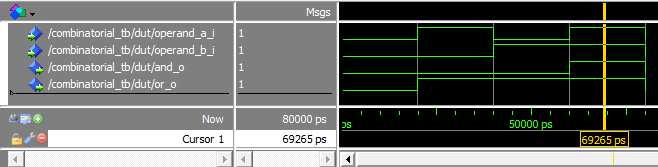
\includegraphics[width=\textwidth]{images/combinatorialSim.png}
    \caption{Waveforms for combinatorial circuit}
    \label{fig:comb-wav}
\end{figure}

\textbf{Result}

The truthtable of an AND and an OR can be recognized in the Waveform:

\begin{equation*}
\begin{array}{cc|cc}
  a_i & b_i & and_o & or_o\\ \hline
  0 & 0 & 0 & 0 \\
  0 & 1 & 0 & 1 \\
  1 & 0 & 0 & 1 \\
  1 & 1 & 1 & 1 \\
\end{array}
\end{equation*}
    
\newpage


\section{Adder}\label{section:adder}

\begin{highlightblock}[Adder]
Write an entity and architecture for the system described in Figure \ref{fig:add}. This entity has two inputs (\vhdl{operand_a_i} and \vhdl{operand_b_i}) and one output. The inputs and outputs of this entity are no single bits but bit vectors (use \vhdl{std_ulogic} vectors). The output \vhdl{result_o} should be calculated as the arithmetical sum of the two inputs. The bit width of the inputs (both should have the same bit width) should be defined by a generic \vhdl{BITWIDTH}. The output bit width should also be defined via this generic (but is of course not equal to this generic...).
\begin{center}
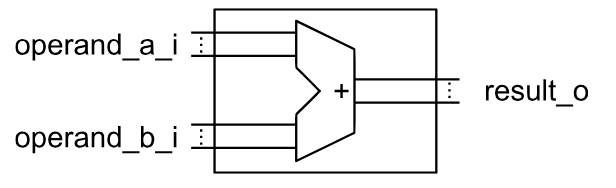
\includegraphics[width=0.5\linewidth]{images/adder.png}

Figure \refstepcounter{figure}\arabic{figure}: Adder\label{fig:add}
\end{center}

\textbf{To-Do-List}

\begin{itemize}
\item Write the entity and the architecture of the system in VHDL. Use one .vhd file for the entity and one .vhd file for the architecture. Describe: how you have defined the output bit width? Give the reasons (few sentences) for your definition.
\item Write a testbench in VHDL (extra file). Test the system and hand in screenshots showing the output of the waveform window. Do two tests with different bit widths ($\leq$ 3 bits). Think of useful test cases (at least 5 different ones for every bit width). In a few sentences summarize the reasons why you have chosen these test cases. In addition do one test where you add two times the maximum value of the inputs. Discuss the result of the simulation in a few sentences. Do you need additional output bits?
\end{itemize}

\end{highlightblock}
\newpage
\subsection{Model Implementation}

Code can be found in the attachments.

\subsection{Simulation}

4-Bit Adder

\begin{center}
    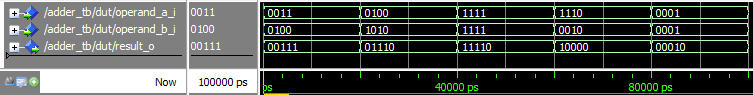
\includegraphics[width=\textwidth]{images/Adder4Sim.png}
\end{center}

12-Bit Adder

\begin{figure}[h]
    \centering
    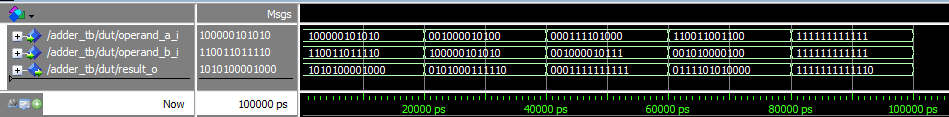
\includegraphics[width=\textwidth]{images/Adder12Sim.png}
    \caption{Caption}
    \label{fig:}
\end{figure}

Die Bitbreite der operanden ist \vhdl{BITWIDTH-1 downto 0} sodass die Breite inklusive der null genau der Bitbreite entspricht. Im Fall des 4-Bit Adder also von 3 bis 0. Beim Ausgang soll das Carry-Bit berück-sichtigt werden, damit die Zahl dargestellt werden kann wenn das Ergebnis die Bitbreite überschreitet. Die größe des resultates ist beim Addierer maximal 1 Bit größer als der größte Eingangswert. Die dimension des resultates ist daher \vhdl{BITWIDTH downto 0}.


Als Testwerte wurden Zahlen verwendet, die unterschiedliche Auswirkungen auf das Carry-Bit haben. Bei der 4-Bit Adder Simulation ist gut zu sehen, wie für beide operanden der höchste 4-Bit Wert 15 gewählt wurde. Wie man sieht, bleibt das resultat innerhalb des definierten Bit-Bereiches


%% 
%%%%%%%%%%%%%%%%%%%%%%%%%%%%%%%%%%%%%%%%%%%%%%%%%%%%%%%%%%%%%%%%%%%%%%%%%%%%%%%%

\end{document}
\endinput
